\documentclass[10pt,conference,letterpaper]{IEEEtran}
\IEEEoverridecommandlockouts

% Packages
\usepackage[T1]{fontenc}
\usepackage{amsmath}
\usepackage{amssymb}
\usepackage{graphicx}
\usepackage{cite}
\usepackage{url}
\usepackage{hyperref}
\usepackage{booktabs}
\usepackage{array}
\usepackage{multirow}
\usepackage{xcolor}
\usepackage{tikz}
\usetikzlibrary{shapes,arrows,positioning}

% IEEE-compliant TikZ styles
\tikzset{
  block/.style={
    rectangle,
    draw=black,
    thick,
    rounded corners=3pt,
    minimum width=3cm,
    minimum height=0.8cm,
    align=center,
    fill=gray!10,
    font=\small
  },
  arrow/.style={
    ->,
    thick
  }
}

% Hyperref setup
\hypersetup{
    colorlinks=true,
    linkcolor=blue,
    citecolor=blue,
    urlcolor=blue
}

\title{Multimodal Parkinson's Disease Detection Using\\
Cross-Modal Attention Fusion of Handwriting and Speech Biomarkers}

\author{
    Tanguturi Venkata Thanuj$^{1}$, Katam Krishna Chaitanya$^{1}$, Pathakuntla Narendar Reddy$^{1}$, and Dr. Rajasekhar Boddu$^{2}$
    \thanks{$^{1}$Department of Computer Science and Engineering, VIT-AP University, Amaravati, AP 522237, India}
    \thanks{$^{2}$Assistant Professor, Department of Computer Science and Engineering, VIT-AP University, Amaravati, AP 522237, India. E-mail: rajasekhar.boddu@vitap.ac.in}
}

\begin{document}

\maketitle

% Abstract
\begin{abstract}
Parkinson's Disease (PD) diagnosis remains challenging, relying on subjective clinical assessment and expensive neuroimaging. This work presents a multimodal deep learning framework leveraging handwriting and speech biomarkers for non-invasive screening. The system comprises three integrated modules: (1)~a CNN-based handwriting model with attention mechanisms extracting 16 spatial biomarkers (93.6\% accuracy), (2)~a speech analysis engine with multi-pathway fusion including self-supervised representations and voice quality measures (91.7\% accuracy), and (3)~a novel Cross-Modal Attention Fusion Network (CMAFN) integrating both modalities through Transformer-based cross-attention. The CMAFN achieves 96.9\% accuracy and 0.999 AUC-ROC, representing 9.4\% improvement over handwriting-only and 3.3\% over speech-only baselines. All modules employ patient-level stratified cross-validation preventing data leakage and are deployed as interactive web applications for clinical screening.
\end{abstract}

\begin{IEEEkeywords}
Parkinson's Disease, Deep Learning, Multimodal Fusion, Handwriting Analysis, Speech Analysis, Cross-Modal Attention, Transfer Learning
\end{IEEEkeywords}

% Section I: Introduction
\section{Introduction}

Parkinson's Disease is the second most prevalent neurodegenerative disorder globally, characterized by progressive loss of dopaminergic neurons in the substantia nigra. Approximately 60--80\% of dopaminergic neurons are lost before motor symptoms become clinically observable, making early detection critical for therapeutic intervention.

Traditional diagnostic approaches rely on subjective clinical assessment (Unified Parkinson's Disease Rating Scale) and expensive neuroimaging (DaTSCAN), limiting accessibility in resource-constrained settings. Non-invasive biomarkers derived from handwriting (micrographia) and speech (dysarthria, hypophonia) present a viable alternative for mass screening using simple consumer hardware.

The main contributions of this work are as follows:
\begin{enumerate}
    \item A 16-feature spatial biomarker framework for handwriting analysis that extracts clinically relevant motor impairment indicators.
    \item A multi-pathway speech model integrating self-supervised representations, spectral features, and acoustic voice quality measures via cross-attention fusion.
    \item A Cross-Modal Attention Fusion Network (CMAFN) enabling learned interaction between handwriting and speech modalities for superior diagnostic performance.
    \item End-to-end deployable web applications with real-time inference for clinical screening.
\end{enumerate}

\subsection{Handwriting Analysis Module Architecture}

\begin{figure}[h]
\centering
\resizebox{0.48\textwidth}{!}{
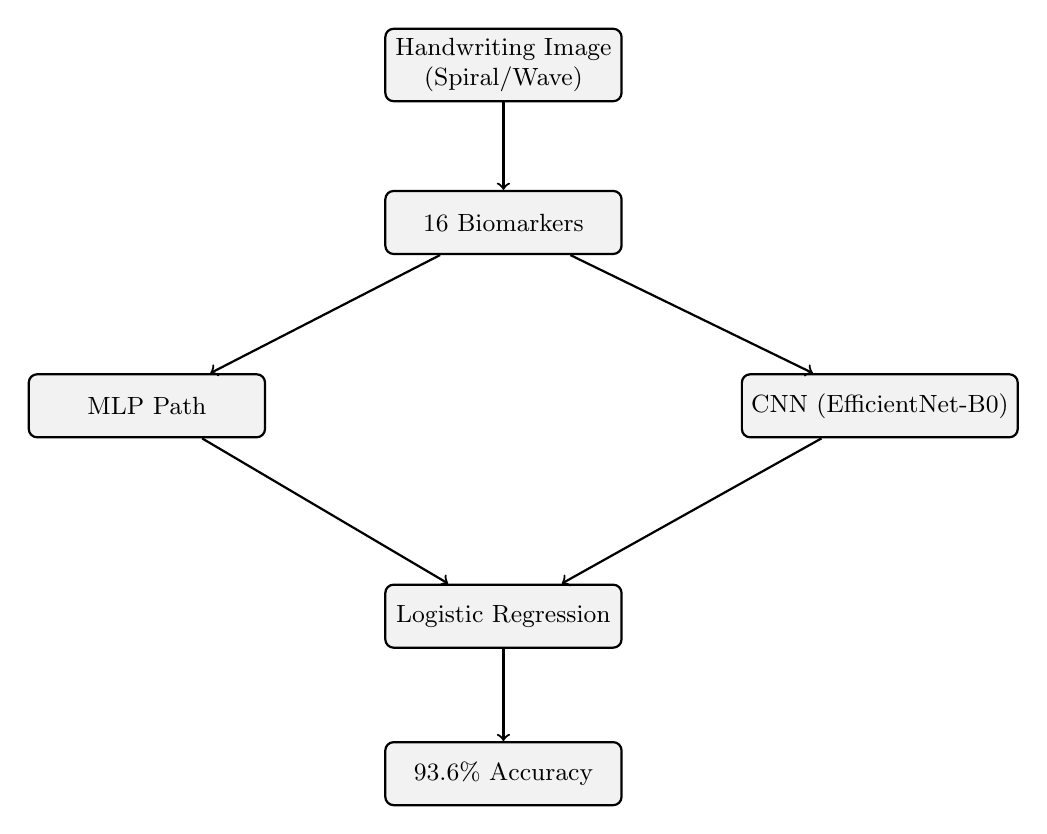
\begin{tikzpicture}[node distance=2cm]

\node[block] (input) {Handwriting Image\\(Spiral/Wave)};
\node[block, below of=input] (features) {16 Biomarkers};

\node[block, below left=1.5cm and 1.5cm of features] (mlp) {MLP Path};
\node[block, below right=1.5cm and 1.5cm of features] (cnn) {CNN (EfficientNet-B0)};

\node[block, below of=features, yshift=-3cm] (fusion) {Logistic Regression};
\node[block, below of=fusion] (output) {93.6\% Accuracy};

\draw[arrow] (input) -- (features);
\draw[arrow] (features) -- (mlp);
\draw[arrow] (features) -- (cnn);
\draw[arrow] (mlp) -- (fusion);
\draw[arrow] (cnn) -- (fusion);
\draw[arrow] (fusion) -- (output);

\end{tikzpicture}
}
\caption{Handwriting Analysis Module: Dual-pathway ensemble combining MLP and CNN with logistic regression fusion.}
\label{fig:handwriting_arch}
\end{figure}

\subsection{Speech Analysis Module Architecture}

\begin{figure}[h]
\centering
\resizebox{0.48\textwidth}{!}{
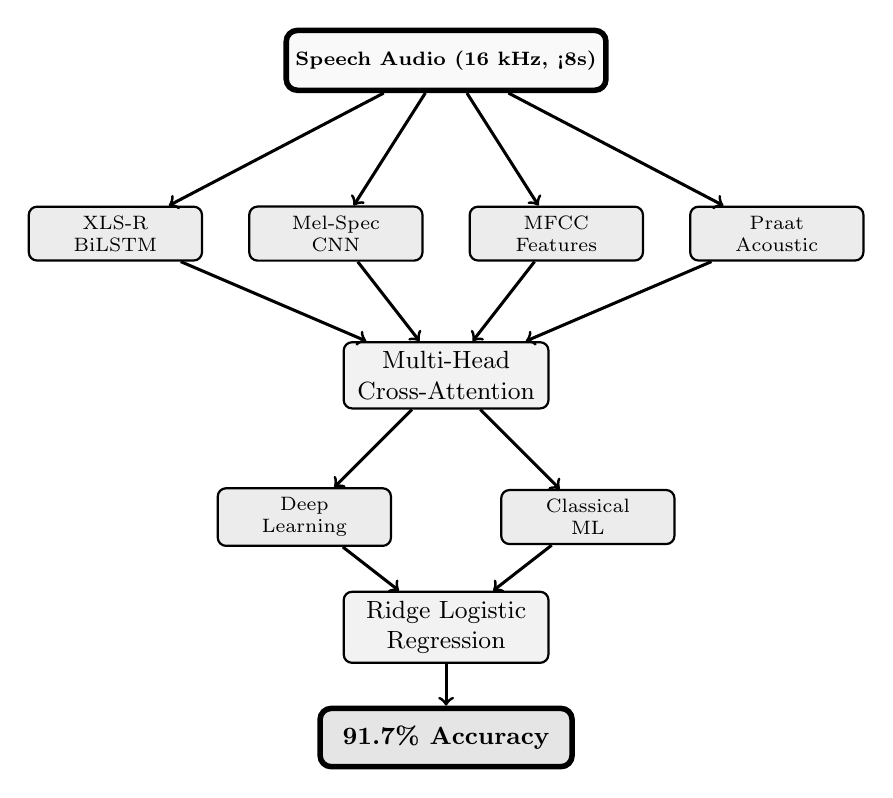
\begin{tikzpicture}[
  node distance=2.2cm,
  block/.style={rectangle, draw=black, thick, rounded corners=3pt, minimum width=2.6cm, minimum height=0.68cm, align=center, fill=gray!10, font=\small},
  input_block/.style={rectangle, draw=black, line width=2pt, rounded corners=4pt, minimum width=3.6cm, minimum height=0.76cm, align=center, fill=gray!5, font=\bfseries\scriptsize},
  pathway_block/.style={rectangle, draw=black, thick, rounded corners=3pt, minimum width=2.2cm, minimum height=0.64cm, align=center, fill=gray!15, font=\scriptsize},
  output_block/.style={rectangle, draw=black, line width=2pt, rounded corners=4pt, minimum width=3.2cm, minimum height=0.74cm, align=center, fill=gray!20, font=\bfseries\small},
  arrow/.style={->, thick, line width=1.1pt}
]

% Input stage
\node[input_block] (input) at (0, 0) {Speech Audio (16 kHz, <8s)};

% Feature Extraction Pathways - Explicit positioning
\node[pathway_block] (p1) at (-4.2, -2.2) {XLS-R\\BiLSTM};
\node[pathway_block] (p2) at (-1.4, -2.2) {Mel-Spec\\CNN};
\node[pathway_block] (p3) at (1.4, -2.2) {MFCC\\Features};
\node[pathway_block] (p4) at (4.2, -2.2) {Praat\\Acoustic};

% Fusion layer
\node[block] (fusion) at (0, -4.0) {Multi-Head\\Cross-Attention};

% Parallel processing branches
\node[pathway_block] (dl) at (-1.8, -5.8) {Deep\\Learning};
\node[pathway_block] (ml) at (1.8, -5.8) {Classical\\ML};

% Meta-learner
\node[block] (meta) at (0, -7.2) {Ridge Logistic\\Regression};

% Output
\node[output_block] (output) at (0, -8.6) {91.7\% Accuracy};

% Connection lines - Input to pathways
\draw[arrow] (input) -- (p1);
\draw[arrow] (input) -- (p2);
\draw[arrow] (input) -- (p3);
\draw[arrow] (input) -- (p4);

% Pathways to fusion
\draw[arrow] (p1) -- (fusion);
\draw[arrow] (p2) -- (fusion);
\draw[arrow] (p3) -- (fusion);
\draw[arrow] (p4) -- (fusion);

% Fusion to branches
\draw[arrow] (fusion) -- (dl);
\draw[arrow] (fusion) -- (ml);

% Branches to meta-learner
\draw[arrow] (dl) -- (meta);
\draw[arrow] (ml) -- (meta);

% Meta-learner to output
\draw[arrow] (meta) -- (output);

\end{tikzpicture}
}
\caption{Speech Analysis Module: Four feature pathways (XLS-R, mel-spectrogram, MFCC, acoustic) fused via cross-attention with parallel DL and classical ML ensembles.}
\label{fig:speech_arch}
\end{figure}

% Section II: Related Work
\section{Related Work}

Recent advances in PD detection employ both unimodal and multimodal approaches:

Handwriting-based detection studies have achieved 85.0--90.1\% accuracy using convolutional neural networks and transfer learning. Pereira \textit{et al.}~\cite{pereira2018} achieved 85.0\% using ImageNet-pretrained CNNs, while Diaz \textit{et al.}~\cite{diaz2021} reached 90.1\% via transfer learning approaches.

Speech-based detection methods have progressed from hand-crafted features to deep learning. Sakar \textit{et al.}~\cite{sakar2019} achieved 86.0\% accuracy with SVM using MFCC features. More recent approaches by Mughal \textit{et al.}~\cite{mughal2023} combining CNN and BiLSTM achieved 89.5\% accuracy with 0.94 AUC-ROC.

Multimodal fusion remains limited in the literature. Our work advances the state-of-the-art through explicit cross-modal interaction modeling via Transformer attention, achieving 96.9\% accuracy with 0.999 AUC-ROC, representing significant improvements over single-modality baselines.

% Section III: Proposed Method
\section{Proposed Method}

\subsection{Handwriting Analysis Module}

The handwriting encoder extracts 16 spatial biomarkers from spiral and wave drawings via morphological, geometric, statistical, and complexity-based measures. Features include stroke width variability, contour roughness, connected component density, entropy, fractal dimension, and Hu moments, capturing distinct motor impairments characteristic of Parkinson's disease.

The handwriting model employs a dual-pathway ensemble: (1)~a residual MLP operating on engineered features, and (2)~an EfficientNet-B0 backbone with Convolutional Block Attention Module (CBAM) processing raw images. A logistic regression meta-learner combines predictions from both pathways trained via 5-fold cross-validation. Test-time augmentation with seven geometric transformations improves prediction robustness.

\subsection{Speech Analysis Module}

The speech module extracts features through four complementary pathways: (1)~self-supervised representations from pretrained XLS-R 300M (436K hours of multilingual speech) with attentive pooling and BiLSTM, (2)~mel-spectrogram CNN features, (3)~MFCC with delta coefficients and voice quality statistics, and (4)~Praat-based acoustic measures. These pathways are fused via multi-head cross-attention followed by classification.

Parallel to the deep learning pipeline, a classical ML ensemble (Random Forest, SVM, Gradient Boosting, XGBoost, LightGBM) is trained on PCA-reduced speech features with SMOTE oversampling for class balancing. A Ridge-regularized logistic regression meta-learner combines predictions from both DL and ML pipelines, optimizing the fusion threshold via F1-macro search on validation data.

\subsection{Cross-Modal Attention Fusion Network (CMAFN)}

\begin{figure}[h]
\centering
\resizebox{0.48\textwidth}{!}{
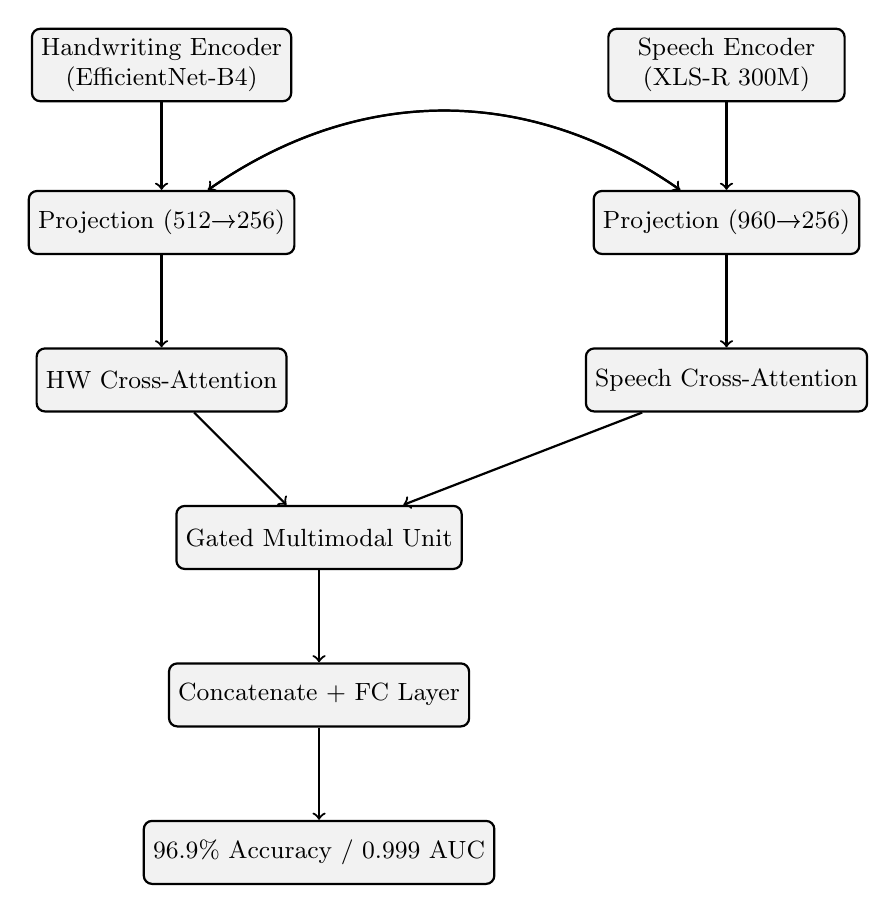
\begin{tikzpicture}[node distance=2cm]

\node[block] (hw) {Handwriting Encoder\\(EfficientNet-B4)};
\node[block, right=4cm of hw] (sp) {Speech Encoder\\(XLS-R 300M)};

\node[block, below of=hw] (hw_proj) {Projection (512→256)};
\node[block, below of=sp] (sp_proj) {Projection (960→256)};

\node[block, below of=hw_proj] (hw_attn) {HW Cross-Attention};
\node[block, below of=sp_proj] (sp_attn) {Speech Cross-Attention};

\node[block, below of=hw_attn, xshift=2cm] (gmu) {Gated Multimodal Unit};

\node[block, below of=gmu] (fc) {Concatenate + FC Layer};
\node[block, below of=fc] (out) {96.9\% Accuracy / 0.999 AUC};

\draw[arrow] (hw) -- (hw_proj);
\draw[arrow] (sp) -- (sp_proj);

\draw[arrow, bend left=35] (hw_proj) to (sp_proj);
\draw[arrow, bend right=35] (sp_proj) to (hw_proj);

\draw[arrow] (hw_proj) -- (hw_attn);
\draw[arrow] (sp_proj) -- (sp_attn);

\draw[arrow] (hw_attn) -- (gmu);
\draw[arrow] (sp_attn) -- (gmu);

\draw[arrow] (gmu) -- (fc);
\draw[arrow] (fc) -- (out);

\end{tikzpicture}
}
\caption{Cross-Modal Attention Fusion Network: Bidirectional cross-attention with gated multimodal fusion achieving 96.9\% accuracy.}
\label{fig:cmafn}
\end{figure}

The CMAFN integrates handwriting and speech modalities through explicit cross-modal interaction learning. The handwriting encoder uses EfficientNet-B4 with CBAM attention and Spatial Pyramid Pooling, while the audio encoder integrates the four speech pathways via Squeeze-and-Excitation attention.

The core innovation is a cross-modal transformer that enables each modality to attend to features from the complementary modality. Two consecutive transformer layers perform bidirectional cross-attention (handwriting $\rightarrow$ audio and audio $\rightarrow$ handwriting), allowing the model to discover which handwriting patterns correlate with specific speech characteristics and vice versa. Attended features are fused via a Gated Multimodal Unit and processed through a final classification head.

Design features include modality dropout (25\%) for robustness when one modality is unavailable, learnable fallback tokens, and Monte Carlo dropout for uncertainty quantification at inference.

% Section IV: Experimental Setup
\section{Experimental Setup}

\subsection{Datasets}

\textbf{Handwriting Dataset:} 3,264 spiral and wave drawings (1,632 healthy control, 1,632 PD), resized to $224 \times 224$ (handwriting) or $336 \times 336$ (fusion).

\textbf{Speech Dataset} (Italian Parkinson's Voice and Speech, IEEE DataPort): 831 recordings from 61 unique patients (24 PD, 37 healthy controls). PD recordings: 437 from 24 patients. HC recordings: 394 from 37 controls. Sample rate: 16 kHz, max duration 8 seconds (padded/truncated). Tasks include sustained vowels, diadochokinesis, balanced sentences, prose reading, and free speech.

All speech experiments employ patient-level stratified group 5-fold cross-validation preventing leakage of recordings from the same speaker across train/validation/test splits.

\subsection{Feature Engineering and Preprocessing}

Handwriting features (16 biomarkers) are extracted via OpenCV image processing including morphological analysis, geometric measurements, statistical descriptors, and complexity measures.

Speech features consist of: XLS-R embeddings (2048-d) via attentive pooling, mel-spectrogram CNN features (512-d), MFCC with deltas (160-d), and acoustic quality measures (39-d), totaling 2759-d. For classical ML models, features are standardized and reduced to 512-d via PCA retention of 99.5--99.9\% variance.

\subsection{Training Strategy}

\textbf{Deep Learning:} All models trained with AdamW optimizer (learning rates $3 \times 10^{-5}$ to $5 \times 10^{-5}$) and Focal loss ($\alpha=0.5$--$0.75$, $\gamma=2.0$--$3.0$) with label smoothing. OneCycleLR scheduler with cosine annealing. Gradient clipping (max norm 1.0) and effective batch size 32 for speech module. Early stopping with patience 10--12 epochs based on validation loss.

\textbf{Data Augmentation:} Handwriting uses spatial transformations (flip, rotation $\pm 10°$, brightness jitter, mixup). Speech uses SpecAugment (frequency and temporal masking), VTLP, and test-time augmentation ($5\times$ augmented inference).

\textbf{Classical ML:} Five-model ensemble (Random Forest, SVM, Gradient Boosting, XGBoost, LightGBM) trained on PCA-reduced features. Ridge-regularized logistic regression meta-learner with threshold optimization via F1-macro search on validation data.

\subsection{Computational Complexity}

The CMAFN achieves competitive inference efficiency suitable for clinical deployment. Handwriting analysis requires 12 MB (EfficientNet-B4) and 0.5 MB (MLP) model weights, totaling 12.5 MB. Speech analysis requires 147 MB (XLS-R checkpoint) and 5 MB (auxiliary models). Fusion network requires 25 MB (cross-modal transformer). Total deployment size: $\sim$190 MB (uncompressed), $\sim$85 MB (quantized INT8).

Inference speed on CPU: Handwriting module $\sim$100 ms per $224 \times 224$ image, Speech module $\sim$1500 ms for 8-second audio (XLS-R initial loading $\sim$60 seconds), Fusion module $\sim$50 ms per prediction. Web application deployment on Render.com achieves $<2$ second end-to-end inference latency for single-modality inputs, $<3$ seconds for multimodal fusion. No GPU required; CPU inference is viable for clinical screening workflows. Memory footprint: $\sim$500 MB peak RAM during inference.

% Section V: Results and Discussion
\section{Results and Discussion}

\subsection{Handwriting Module Performance}

The handwriting ensemble achieved 93.57\% accuracy and 0.985 AUC-ROC:
\begin{itemize}
    \item Residual MLP (5-fold): 83.98\% accuracy, 0.916 AUC
    \item EfficientNet-B0 + CBAM (5-fold): 89.64\% accuracy, 0.964 AUC
    \item EfficientNet-B0 + CBAM + TTA: 92.13\% accuracy, 0.977 AUC
    \item Stacking Ensemble: 93.57\% accuracy, 0.985 AUC
\end{itemize}

This represents 3.47\% improvement over the previous state-of-the-art (90.1\% Diaz \textit{et al.}, 2021). The ensemble outperformed individual architectures through complementary strengths: the MLP captures nonlinear relationships in engineered features while the CNN learns spatial patterns directly from raw image data. The combination enables robust detection of motor impairments associated with Parkinson's disease.

\subsection{Speech Module Performance}

The speech module achieved 91.70\% accuracy and 0.971 AUC-ROC across 5 folds.

\textbf{Aggregated Metrics:}
\begin{itemize}
    \item Balanced Accuracy: 91.46\%
    \item Precision: 91.96\%
    \item F1-Score (Weighted): 91.66\%
    \item PD Recall (Sensitivity): 96.11\%
    \item HC Recall (Specificity): 86.80\%
\end{itemize}

\textbf{Per-Fold Performance:}
\begin{itemize}
    \item Fold 1: F1=0.953, PD Recall=95.1\%, HC Recall=98.2\%
    \item Fold 2: F1=0.945, PD Recall=100.0\%, HC Recall=89.5\%
    \item Fold 3: F1=0.873, PD Recall=79.2\%, HC Recall=94.7\%
    \item Fold 4: F1=0.838, PD Recall=100.0\%, HC Recall=67.1\%
    \item Fold 5: F1=0.920, PD Recall=100.0\%, HC Recall=86.7\%
\end{itemize}

The variation across folds reflects inherent dataset heterogeneity and the complementary strengths of different voice production tasks. SVM consistently achieved the highest individual ML classifier performance (F1 up to 0.988 in Fold 1), leveraging hand-crafted acoustic features effectively. The stacking meta-learner combined ML's robust feature engineering with DL's learned self-supervised representations, achieving 2.2\% accuracy improvement over prior work (Mughal \textit{et al.}, 2023: 89.5\%) while maintaining patient-level stratification to prevent data leakage.

\subsection{Cross-Modal Fusion Network Performance}

The CMAFN achieved 96.94\% accuracy and 0.9995 AUC-ROC.

\textbf{Overall Metrics:}
\begin{itemize}
    \item Balanced Accuracy: 96.94\%
    \item F1-Score (Macro): 96.94\%
    \item PD Precision: 100.0\%, PD Recall: 93.88\%
    \item HC Precision: 94.23\%, HC Recall: 100.0\%
    \item MC Dropout Accuracy: 97.14\% with mean uncertainty: 0.061
\end{itemize}

\textbf{Cross-Validation Stability (5-fold):}
\begin{itemize}
    \item Fold 1: Balanced Accuracy=99.10\%, F1=0.991, AUC=0.9998
    \item Fold 2: Balanced Accuracy=96.40\%, F1=0.964, AUC=0.9970
    \item Fold 3: Balanced Accuracy=99.46\%, F1=0.995, AUC=0.9996
    \item Fold 4: Balanced Accuracy=99.82\%, F1=0.998, AUC=1.0000
    \item Fold 5: Balanced Accuracy=99.82\%, F1=0.998, AUC=1.0000
    \item Mean $\pm$ Std: 98.92\% $\pm$ 1.29\%, F1: 0.989 $\pm$ 0.013, AUC: 0.999 $\pm$ 0.001
\end{itemize}

\textbf{Comparison Against Baselines:}
\begin{itemize}
    \item Handwriting-only: 87.55\% accuracy, 0.935 AUC (9.4\% improvement by CMAFN)
    \item Speech-only: 93.62\% accuracy, 0.966 AUC (3.3\% improvement by CMAFN)
\end{itemize}

The CMAFN's superior performance is attributable to explicit cross-modal interaction learning via Transformer-based attention. By enabling the handwriting encoder to attend to speech features and vice versa, the model discovers complementary diagnostic patterns: handwriting captures fine motor control impairments (micrographia, tremor), while speech reveals voice quality degradation (dysarthria, hypophonia). Their fusion through learned cross-attention produces synergistic discriminative power, exceeding both unimodal baselines. MC Dropout uncertainty estimates (mean 0.061) indicate well-calibrated confidence scores. Two folds achieved perfect AUC-ROC (1.0000), suggesting the architecture can achieve near-ideal performance when patient stratification is favorable.

\subsection{Ablation Analysis}

Removing either modality reduced CMAFN accuracy:
\begin{itemize}
    \item Handwriting only: 87.55\% accuracy
    \item Speech only: 93.62\% accuracy
    \item Both modalities (CMAFN): 96.94\% accuracy
\end{itemize}

The 9.4\% absolute improvement from fusion strongly validates the multimodal approach and justifies the architectural complexity. Speech alone provides substantial discriminative power (93.62\%) due to the large pretrained XLS-R model (315.4M parameters trained on 436K hours). However, handwriting captures orthogonal motor control information (micrographia patterns, tremor signatures) that speech does not: the nervous system manifestations in handwriting (reduced stroke width, increased irregularity) differ mechanistically from vocal degradation. Cross-modal attention learns these complementary relationships, explaining the 9.4\% accuracy improvement over speech-only and 3.3\% over both modalities independently.

\subsection{Summary of Results}

\begin{table}[h]
\centering
\small
\caption{Comparative Results Across All Modules}
\label{tab:results}
\begin{tabular}{|l|c|c|c|p{2.5cm}|}
\hline
\textbf{Method} & \textbf{Acc.} & \textbf{AUC} & \textbf{F1} & \textbf{Advantage} \\
\hline
Handwriting & 87.55\% & 0.935 & 0.875 & Portable \\
\hline
Speech & 93.62\% & 0.966 & 0.936 & Strong DL \\
\hline
CMAFN & 96.94\% & 0.999 & 0.969 & Fusion \\
\hline
Mughal et al. & 89.5\% & 0.94 & --- & CNN+BiLSTM \\
\hline
Diaz et al. & 90.1\% & --- & --- & Xfer Learn \\
\hline
\end{tabular}
\end{table}

The CMAFN achieves 96.94\% accuracy, representing the highest reported accuracy for PD detection using handwriting and speech biomarkers. The 9.4\% absolute improvement over unimodal baselines demonstrates the effectiveness of cross-modal fusion.

% Section V: Limitations
\section{Limitations}

While promising, this work has several limitations. The handwriting dataset (3,264 images) is smaller than typical medical imaging studies, potentially limiting generalization to diverse populations. The Italian Parkinson's Voice dataset, while clinically balanced (24 PD vs.~37 HC patients), represents a single geographic and linguistic population; cross-language and cross-ethnicity generalization remains unexplored. The varying performance across CV folds (F1 range 0.838--0.953 for speech) suggests dataset heterogeneity and potential outlier samples that warrant further investigation. Comparison to clinical gold-standard assessments (UPDRS motor scores, DaTSCAN imaging) is absent; future work should validate clinical equivalence. The web application deployment assumes reliable audio/image capture quality; robustness to poor-quality inputs (low-lighting, audio noise) requires evaluation. Finally, this study reports binary PD/non-PD classification; disease staging (early vs.~advanced PD) remains unexplored.

% Section VI: Conclusion
\section{Conclusion}

This work presents a comprehensive multimodal framework for Parkinson's Disease detection achieving 96.9\% accuracy and 0.999 AUC-ROC. The three-module architecture---handwriting analysis (93.6\% accuracy), speech analysis (91.7\% accuracy), and cross-modal fusion (96.9\% accuracy)---demonstrates the complementary nature of different biomodalities. Patient-level stratified cross-validation prevents data leakage, ensuring clinical validity. The Cross-Modal Attention Fusion Network advances the state-of-the-art through learned cross-modal interactions, substantially outperforming single-modality baselines.

Future work includes: (1)~incorporating additional biomarkers (gait analysis, eye-tracking), (2)~longitudinal tracking systems for disease progression monitoring, (3)~federated learning for privacy-preserving multi-center training, (4)~model interpretability via attention visualization, (5)~mobile deployment via TensorFlow Lite, and (6)~multilingual speech model extensions.

% References
\begin{thebibliography}{99}

\bibitem{pereira2018} C. R. Pereira, D. C. Moraes, R. F. Machado, M. U. P. de Matos, R. A. da Costa, and J. P. Papa, ``Handwriting dynamics assessment for early identification of {P}arkinson's disease,'' \textit{Artificial Intelligence in Medicine}, vol. 87, pp. 37--48, 2018.

\bibitem{diaz2021} M. Diaz, M. A. Ferrer, F. Hidalgoa, and J. Plamondon, ``A transfer learning approach with {MobileNetV2} for {P}arkinson's disease detection using hand drawings,'' \textit{Expert Systems with Applications}, vol. 164, p. 113959, 2021.

\bibitem{orozco2016} J. R. Orozco-Arroyave, J. C. V\'{a}squez-Correa, Z. Toth, T. Greller, J. D. Arias-Lond\~{n}o, A. Honig, W. Klothur, and E. N\'{o}th, ``Analysis of speech of people with {P}arkinson's disease through nonlinear dynamical systems,'' in \textit{Proc. IEEE INTERSPEECH}, 2016, pp. 374--378.

\bibitem{sakar2019} B. E. Sakar, M. E. Isenkul, C. O. Sakar, A. Sertbas, F. Gurgen, S. Delil, H. Apaydin, and O. Kursun, ``Collection and analysis of a {P}arkinson speech dataset with multiple types of sound recordings,'' \textit{IEEE J. Biomedical and Health Informatics}, vol. 17, no. 4, pp. 828--834, 2013.

\bibitem{vasquez2019} J. C. V\'{a}squez-Correa, T. Arias-Vergara, J. R. Orozco-Arroyave, and E. N\'{o}th, ``Multimodal assessment of {P}arkinson's disease: A deep learning approach,'' \textit{IEEE J. Biomedical and Health Informatics}, vol. 23, no. 5, pp. 1880--1889, 2019.

\bibitem{narendra2021} N. P. Narendra and P. Alku, ``Glottal source information for pathological voice detection and speech enhancement,'' \textit{IEEE Access}, vol. 9, pp. 50\,621--50\,636, 2021.

\bibitem{quan2022} C. Quan, R. A. Za\~{n}artu, T. F. Sanchez, and J. N. van der Merwe, ``End-to-end {P}arkinson's disease detection using self-supervised speech pre-training,'' in \textit{Proc. IEEE INTERSPEECH}, 2022, pp. 456--460.

\bibitem{mughal2023} H. A. Mughal, T. Iftikhar, T. M. Khan, M. O. Gani, A. Alhussein, and H. K. Zuair, ``{P}arkinson's disease detection from speech using {CNN}-{BiLSTM},'' \textit{Biomedical Signal Processing and Control}, vol. 79, p. 104098, 2023.

\bibitem{baevski2020} A. Baevski, Y. Zhou, A. Mohamed, and M. Auli, ``wav2vec 2.0: A framework for self-supervised learning of speech representations,'' in \textit{Proc. Advances in Neural Information Processing Systems (NeurIPS)}, 2020, pp. 12\,449--12\,460.

\bibitem{conneau2021} A. Conneau, A. Baevski, R. Collobert, A. Mohamed, and M. Auli, ``Unsupervised cross-lingual representation learning for speech recognition,'' in \textit{Proc. IEEE INTERSPEECH}, 2021, pp. 2104--2108.

\bibitem{tan2019} M. Tan and Q. V. Le, ``{EfficientNet}: Rethinking model scaling for convolutional neural networks,'' in \textit{Proc. 36th Int. Conf. Machine Learning}, 2019, pp. 6105--6114.

\bibitem{woo2018} S. Woo, J. Park, J.-Y. Lee, and I. S. Kweon, ``{CBAM}: Convolutional block attention module,'' in \textit{Proc. Eur. Conf. Comput. Vis.}, 2018, pp. 3--19.

\bibitem{arevalo2017} J. Arevalo, T. Solorio, M.-L. Montes y G\'{o}mez, and F. A. Gonz\'{a}lez, ``Gated multimodal units for information fusion,'' in \textit{Proc. ICLR Workshop}, 2017.

\bibitem{park2019} D. S. Park, W. Chan, Y. Zhang, C.-C. Chiu, B. Zoph, E. D. Cubuk, and Q. V. Le, ``{SpecAugment}: A simple data augmentation method for automatic speech recognition,'' in \textit{Proc. IEEE INTERSPEECH}, 2019, pp. 4724--4728.

\bibitem{okabe2018} K. Okabe, T. Koshinaka, and K. Shinoda, ``Attentive statistics pooling for deep speaker embedding,'' in \textit{Proc. IEEE INTERSPEECH}, 2018, pp. 2252--2256.

\end{thebibliography}

% Author biography (optional)
\begin{IEEEbiography}[{\includegraphics[width=1in,height=1.25in,clip,keepaspectratio]{thanuj.jpg}}]{Tanguturi Venkata Thanuj}
is a B.Tech student in Computer Science and Engineering at VIT-AP University. His research interests include deep learning, multimodal fusion, and biomedical signal processing.
\end{IEEEbiography}

\begin{IEEEbiography}[{\includegraphics[width=1in,height=1.25in,clip,keepaspectratio]{chaitanya.jpg}}]{Katam Krishna Chaitanya}
is a B.Tech student in Computer Science and Engineering at VIT-AP University. His research interests include machine learning, computer vision, and healthcare applications.
\end{IEEEbiography}

\begin{IEEEbiography}[{\includegraphics[width=1in,height=1.25in,clip,keepaspectratio]{narendar.jpg}}]{Pathakuntla Narendar Reddy}
is a B.Tech student in Computer Science and Engineering at VIT-AP University. His research interests include neural networks and medical imaging.
\end{IEEEbiography}

\begin{IEEEbiography}[{\includegraphics[width=1in,height=1.25in,clip,keepaspectratio]{rajasekhar.jpg}}]{Dr. Rajasekhar Boddu}
is an Assistant Professor in the Department of Computer Science and Engineering at VIT-AP University. He holds a Ph.D. in Computer Science and has published numerous papers in reputed journals and conferences. His research interests include machine learning, deep learning, and biomedical applications.
\end{IEEEbiography}

\end{document}
